%
%
% 	Пример 03
%

%
%	С этой команды начинается каждый документ LaTeX: она задаёт общие настройки формата документа
%	Формат бумаги А4, 12й кегль (размер шрифта)
%
\documentclass[a4paper,12pt]{article}

%
%	Эти две команды подключают локализацию
%
\usepackage[utf8]{inputenc}			% Кодировка символов --- Юникод.
\usepackage[english, russian]{babel}		% Язык: шрифты, переносы и т.д.

%
%	Эти команды регулируют внешний вид документа
%

\usepackage{indentfirst}	% Абзацный отступ после начала глав и разделов
\usepackage{a4wide}		% Сужает поля

%
%	Эти команды подключают много полезного для работы с формулами
%

\usepackage{amsmath}
\usepackage{amsthm}
\usepackage{amssymb}

%
%	Пакеты для картинок
%
\usepackage[dvips]{graphicx}
\usepackage{float}

%
%	Основное тело документа
%
\begin{document}

\begin{figure}[T]
 \centering % выравнивание по центру
 %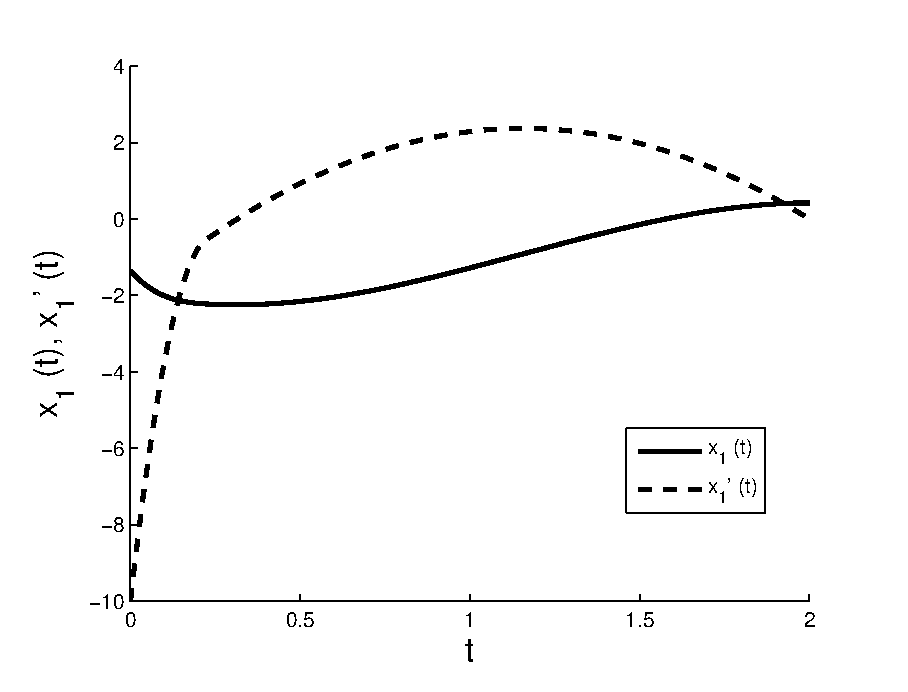
\includegraphics[keepaspectratio, width=0.8\textwidth]{pic_01}
\caption{hi!}

\end{figure}

\begin{figure}
 \centering % выравнивание по центру
 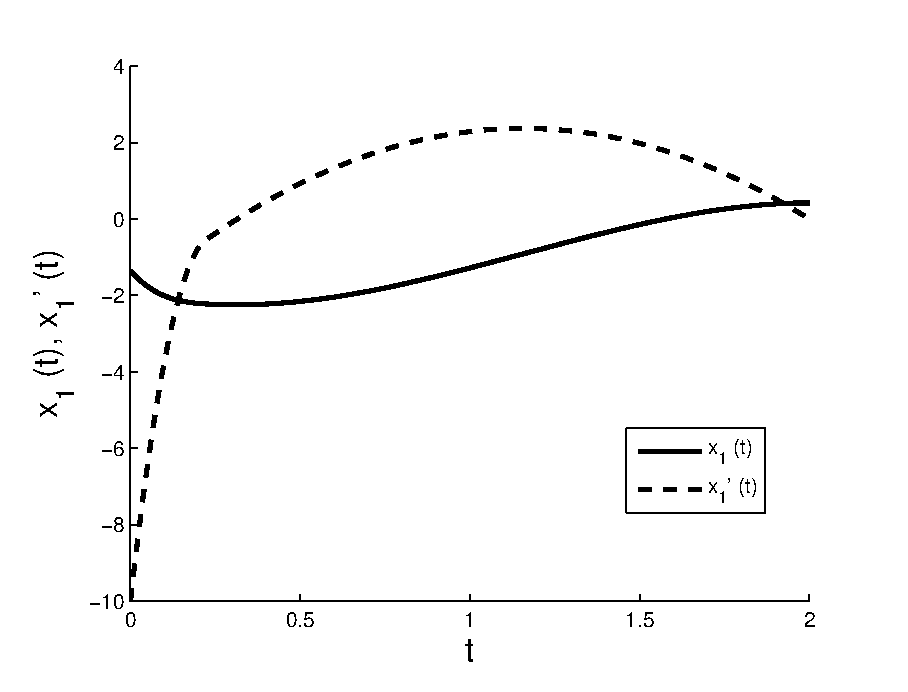
\includegraphics[keepaspectratio, width=0.45\textwidth]{pic_01}


 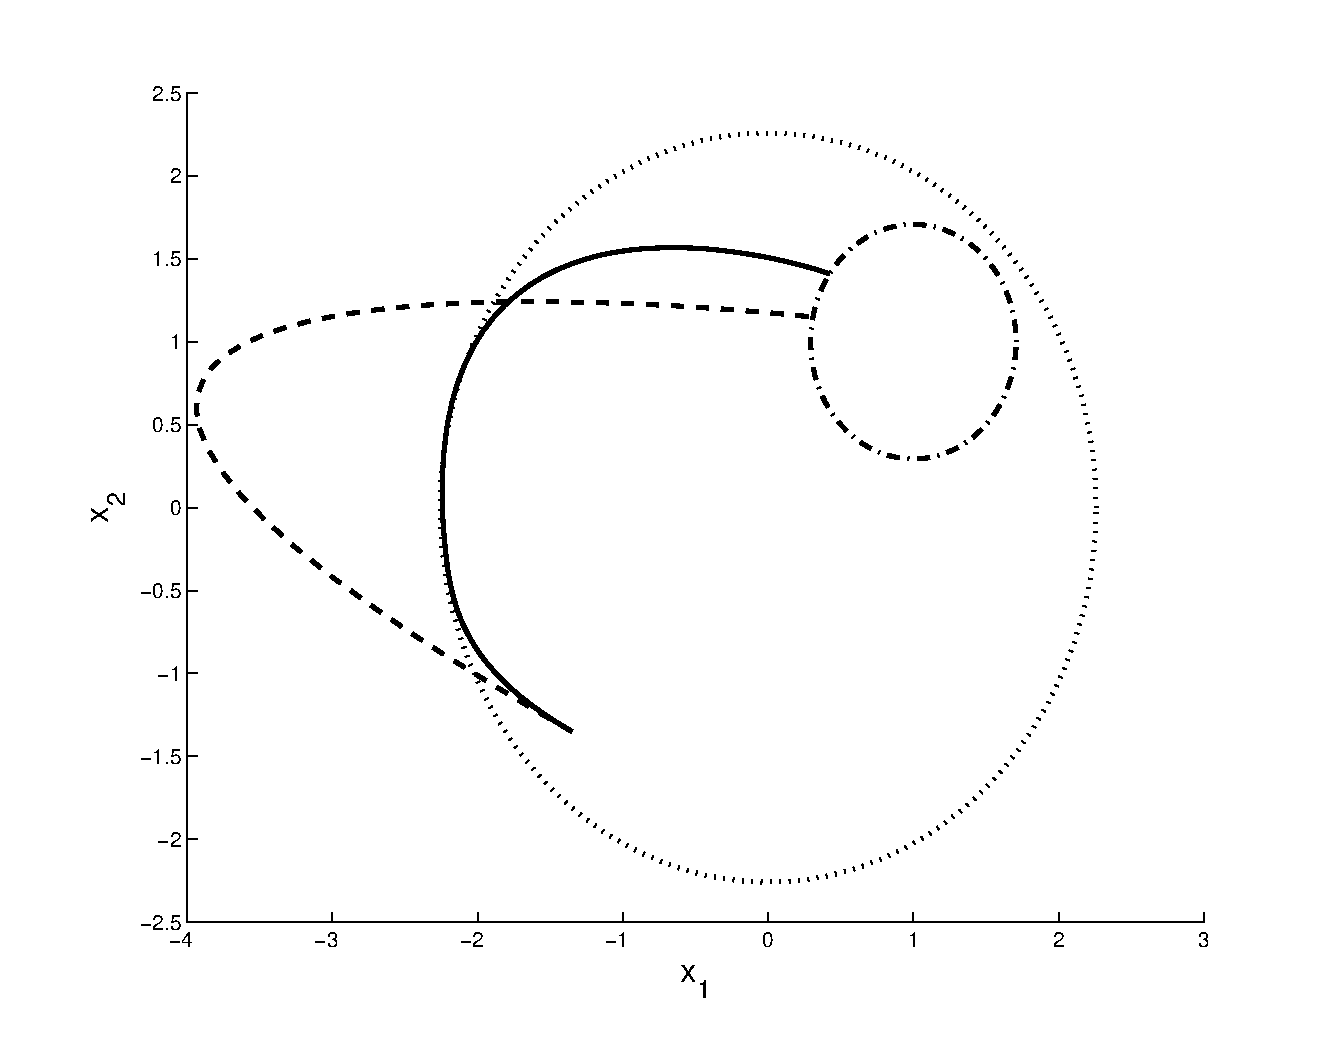
\includegraphics[keepaspectratio, width=0.45\textwidth]{pic_02}
\caption{Две картинки!}\label{dataPic}
\end{figure}

На рисунке \ref{dataPic} изображено два графика.


\end{document} 
